\clearpage
\section{UV-Fixpunkte der $SU_\text{QCD}\times SU_\text{dQCD}$}\label{beta_QCDxdQCD}

  Die allgemeinste Form der $\beta$-Funktion auf 2-Schleifen Ordnung 
  einer $G_1\times G_2$-Eichtheorie wurde von 
  D.R.T. Jones berechnet \cite{Jones}. Angewand auf die $SU(\Nc)\times SU(\Nd)$ ergibt 
  sich für 
  die $\beta$-Funktion die Form
  \begin{equation}
   \begin{pmatrix}
   \beta_\s\\ \beta_\d
   \end{pmatrix}
    = \begin{pmatrix}
                     X_\s^g g_\s^3 + Y_\s^g g_\s^5 + Z_\s^g g_\s^3 g_\d^2 \\ 
                     X_\d^g g_\d^3 + Y_\d^g g_\d^5 + Z_\d^g g_\d^3 g_\s^2 
                    \end{pmatrix}\quad . \label{eq:beta_QCDxdQCD:beta_g}
  \end{equation}
  Für die Darstellungen $R_\s$, $R_\d$, $S_\s$ und $S_\d$ der Fermionen bzw. Skalare 
  sind die Koeffizienten von $\beta_\s$ gegeben durch 
  \begin{align}
   X_\s^g &= (16 \uppi^2)^{-1}\left[ \frac{2}{3} T(R_\s) d(R_\d) + \frac{1}{3} 
    T(S_\s)d(S_\d)-\frac{11}{3} C_2(SU(\Nc)) \right] \label{eq:beta_QCDxdQCD:X1}\\
    \begin{split}
   Y_\s^g &= (16 \uppi^2)^{-2} \left[ 
    \left( 
    \frac{10}{3} C_2(SU(\Nc))+2C_2(R_\s)
    \right) T(R_\s) d(R_\d) \right. \\
     & \quad \quad \quad \quad \quad + \left. \left(
    \frac{2}{3} C_2(SU(\Nc)) +4C_2(S_\s) 
    \right)T(S_\s) d(S_\d)
    -\frac{34}{3} C_2(SU(\Nc))^2
    \right] \label{eq:beta_QCDxdQCD:Y1}
    \end{split}\\
   Z_\s^g &= (16 \uppi^2)^{-2} \left[
      2 C_2(R_\d) d(R_\d) T(R_\s) +4C_2(S_\d)d(S_\d) T(S_\s)
    \right] \quad .\label{eq:beta_QCDxdQCD:Z1}
  \end{align}
  Die Berechnung ist für Weyl-Fermionen geschehen. Betrachtet man Dirac-Fermionen 
  erhalten $d(R_\s)$ und $d(R_\d)$ einen zusätzlichen Faktor von $2$. Die 
  Koeffizienten $X_\d^g$, $Y_\d^g$ und $Z_\d^g$ können durch den Tausch 
  $\s \leftrightarrow \d$ erhalten werden.
  Die Darstellungen der beteiligten Quantenfelder in der \QCDxdQCD sind noch einmal 
  in Tabelle \ref{tab:beta_QCDxdQCD:Darstellungen} zusammengefasst.
 \begin{table}
\centering
\begin{tabular}{c|ccccc}
 Eichgruppe	& $\psi$	, $\phi$	&$\xi$, $\chi$	&$\zeta$, $\eta$ & $\A$ & $\widetilde{\A}$ 
 \\
 $SU(\Nc)$	& $\Nc$	& $1$ &$\Nc$ & $\Nc^2-1$ & $1$ \\ 
 $SU(\Nd)$	& $1$	& $\Nd$ &$\Nd$ & $1$ & $\Nd^2-1$ \\
\end{tabular}
\caption{Die Darstellungen der Beteiligten Quantenfelder. Dabei Stellen 
$\psi$ und $\phi$ die Dirac-Fermionen und Skalare der QCD, 
$\xi$ und $\chi$ die der dQCD dar, die Felder $\zeta$ und $\eta$ sind unter beiden 
Eichgruppen geladen. Die Eichbosonen $\A$ und $\widetilde{\A}$ sind in der 
adjungierten Darstellung der QCD bzw. dQCD.}
\end{table}  
 
  In den gewählten Darstellungen gilt $T(R_\s)=T(S_\s)=T(R_\d)=T(S_\s)=1/2$, außerdem  
  $C_2(SU(N_{\s/\d}))=N_{\text{s}/\text{d}}$ sowie 
  $C_2(R_{\s/\d})=C_2(S_{\s/\d})=(N_{\s/\d}^2-1)/(2 N_{\s/\d})$. 
  In der $\text{QCD}\times\text{dQCD}$ gibt es drei 
  verschiedenen Darstellungskombinationen der Materiefelder.   
  Daher können $d(R_\s)$ und $d(R_\d)$ bzw. $d(S_\s)$ und $d(S_\d)$
  in 
  jedem Koeffizienten \eqref{eq:beta_QCDxdQCD:X1}, \eqref{eq:beta_QCDxdQCD:Y1} 
  und \eqref{eq:beta_QCDxdQCD:Z1} andere Werte annehmen und müssen deshalb 
  einzeln bestimmt werden. Dies geschieht am einfachsten über das 
  Zeichnen von Feynmandiagrammen und Abzählen der möglichen Teilchen, die im 
  entsprechenden Diagramm erlaubt sind.


    Die Teilchenlinien in den Diagrammen werden nur mit ihren QCD und dQCD 
    Quantenzahlen 
    beschriftet. Dabei stehen wieder $i$ und $j$ für Colour bzw. $r$ und $s$ für 
    dark Colour in der fundamentalen Darstellung, $A$ und $M$ für Colour und 
    dark Colour der adjungierten Darstellung. Die Vertizes werden mit den 
    entsprechenden Erzeugermatrizen beschriftet und 
    enthalten bereits die Kopplungskonstanten. Es werden nur die Koeffizienten 
    $X_\s^g$, $Y_\s^g$ und $Z_\s^g$ betrachtet, $X_\d^g$, $Y_\d^g$ und $Z_\d^g$ 
    folgen analog mit $\text{QCD}\leftrightarrow \text{dQCD}$. Außerdem werden nur 
    Fermionen diskutiert, um $d(S_{\s})$ zu erhalten muss lediglich $\nfc \to 
    \nsc$ und $\nfj\to \nsj$ ersetzt werden. Das gleiche gilt für $d(S_\d)$.
    Wie in 
    \cite{MACHACEK198383} gezeigt, kann die Eichung des Eichboson-Propagators 
    so gewählt werden, dass die $\beta$-Funktion nur noch von der 
    Renormierungskonstanten $Z_A$ des Eichfeldes abhängt. Daher reicht es, 
    hier nur 1- und 2-Schleifen Korrekturen zum Gluon-Propagator zu untersuchen, 
    Korrekturen zu 3- oder 4-Punkt Funktionen müssen nicht berücksichtigt 
    werden.
    
    Der Koeffizient $X_\s^g$ entspricht der 1-Schleifen Korrektur zum 
    Gluonpropagator. Bei der Fermionschleife in Abbildung 
    \ref{fig:n-schleifen:QCD3} kann jedes der $\nfc$ 
    QCD-Fermionen und jedes der 
    $\nfj$ joint-Fermionen mit einer dark Colour 
    $r\in\{1,2,\ldots,\Nd \}$ in der 
    Schleife auftauchen. Damit ist $d(R_\d)=\nfc+\Nd \nfj$.
    \begin{figure}[h]
\centering
 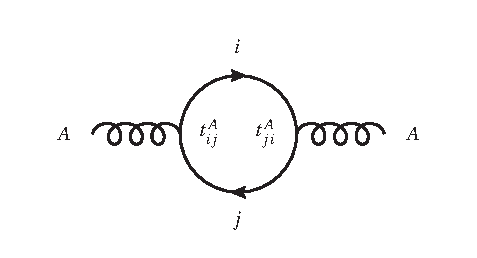
\includegraphics{abschnitte/n-schleifen/fig/QCD3.eps}
 \caption{1-Schleifen QCD/joint-Fermion Beitrag zum Gluonpropagator.}\label{fig:n-schleifen:QCD3}
\end{figure}
    
    Der Koeffizient $Y_\s^g$ enthält die 2-Schleifen Beiträge proportional zu 
    $(t^A_{ij})^4$. Auch hier kann jeweil ein QCD-Fermion oder ein 
    joint-Fermion mit einer dark Colour vorkommen, sodass wieder 
    $d(R_\d)=\nfc+\Nd\nfj$.
    
    Die Diagramme proportional zu $(t^A_{ij})^2(\widetilde{t}^{M}_{rs})^2$ 
    tragen zu $Z_\s^g$ bei und sind in Abbildung 
    \ref{fig:n-schleifen:QCDxdQCD2} zu sehen.
    Am Gluon-Fermion Vertex $t^A_{ij}$ kann $r$ jeden Wert $1,2,\ldots,\Nd$ 
    annehmen, wieder mit jedem Flavour. QCD- oder dQCD-Fermionen können nicht 
    auftauchen, sodass in diesem Fall $d(R_\d)=\Nd \nfj$.
    \begin{figure}[h]
 \centering
 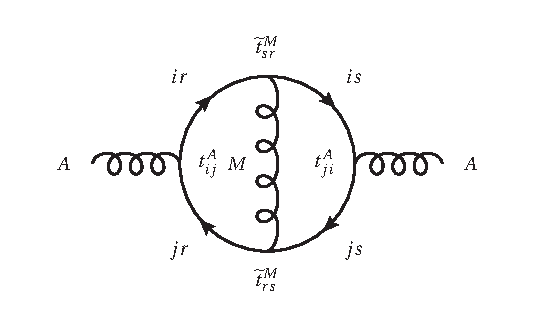
\includegraphics{abschnitte/n-schleifen/fig/QCDxdQCD1.eps}
 \caption{Vertexkorrektur zum Gluonpropagator.}\label{fig:n-schleifen:QCDxdQCD1}
\end{figure}

  
  
  Die ermittelten Koeffizienten stimmen mit denen in \cite{Scale_of_dark_QCD} 
  überein. Mit $\Nfc := \nfc +\Nd \nfj$, $\Nsc := \nsc +\Nd \nsj$, 
  $\Nfd := \nfd +\Nc \nfj$ und $\Nsd := \nsd +\Nc \nfj$ lassen sie sich 
  schreiben als
  \begin{align}
   X_\s^g &= (16 \uppi^2)^{-1} \left[
    \frac{2}{3} \Nfc + \frac{1}{6} \Nsc - \frac{11}{3} \Nc \right] 
    \label{eq:beta_QCDxdQCD:X1g} \\ 
   Y_\s^g &= (16 \uppi^2)^{-2} \left[ \left(\frac{13}{3}\Nc-\frac{1}{\Nc}\right)
    \Nfc + \left( \frac{4}{3} \Nc -\frac{1}{\Nc}\right)\Nsc -\frac{34}{3}
    \Nc^2\right] \label{eq:beta_QCDxdQCD:Y1g}\\
   Z_\s^g &= (16 \uppi^2)^{-2}\left[(\Nd^2-1)(\nfj + \nsj) \right] \quad .
   \label{eq:beta_QCDxdQCD:Z1g}
  \end{align}

  Da beide Kopplungskonstanten in einer $4$-dimensionalen Raumzeit die 
  Massendimension $[g_\s]=[g_\d]=0$ besitzen, werden die neuen 
  Kopplungskonstanten $\alpha_i := \nicefrac{g_i^2}{4 \uppi}$ 
  eingeführt. Die Bedingung $|g_i|<1$ für eine sinnvolle Störungstheorie lässt 
  sich zu $\alpha_i<4\uppi$ übersetzen. Mit 
  $X_i := 8\uppi X_i^g $, $Y_i := 32\uppi^2 Y_i^g $ und 
  $Z_i := 32\uppi^2 Z_i^g $ folgt
  \begin{equation}
   \beta (\alpha) = \begin{pmatrix}
                     X_\s \alpha_\s^2 + Y_\s \alpha_\s^3 + Z_\s \alpha_\s^2 \alpha_\d\\ 
                     X_\d \alpha_\d^2 + Y_\d \alpha_\d^3 + Z_\d \alpha_\s \alpha_\d^2 
                    \end{pmatrix} \label{eq:beta_QCDxdQCD:beta_alpha}
  \end{equation}
  und als Nullstellen findet man den Gaußschen Fixpunkt
   \begin{equation}
   \alpha^{*}_\text{Gauß}=(0,0) \quad , 
   \end{equation}
   die teilweise wechselwirkenden Fixpunkte 
   \begin{equation}
   \alpha^{*}_\text{tw1}=\left(-\frac{X_\s}{Y_\s},0\right) \quad ,
   \alpha^{*}_\text{tw2}=\left(0,-\frac{X_\d}{Y_\d}\right) \quad 
   \end{equation}
   und den vollständig wechselwirkenden Fixpunkt
   \begin{equation}
   \alpha^{*}_\text{vw}=\left(\frac{Z_\s X_\d-X_\s Y_\d}{Y_\s Y_\d-Z_\s Z_\d} ,
	\frac{Z_\d X_\s -X_\d Y_\s}{Y_\s Y_\d - Z_\s Z_\d}\right) \quad . 
	\label{eq:beta_QCDxdQCD:Fixpunkte}
   \end{equation}
  An den Fixpunkten gilt außerdem 
  \begin{equation}
    \left. \Sp \right|_*=(\alpha_\s^*)^2 Y_\s+(\alpha_\d^*)^2 Y_\d
    \quad
    \text{sowie}
    \quad
    \left. \Det \right|_*=(\alpha_\s^*\alpha_\d^*)^2(Y_\s Y_\d - Z_\s Z_\d) \quad.
    \label{eq:beta_QCDxdQCD:spur_determinante}
  \end{equation}
  

  
  \subsection{UV-Verhalten bei $\alpha^{*}_\text{vw}$}
    \subsubsection{attraktiver Fixpunkt}\label{beta_QCDxdQCD:fix4:UV}
      Für komplett UV-attraktives Verhalten müssen die Bedingungen 
      \begin{equation}
      \alpha_\s^* > 0 \quad \land \quad
      \alpha_\d^* > 0 \quad \land \quad
      \left. \Det \right |_* > 0 \quad \land \quad 
      \left. \Sp  \right |_*  < 0 \label{eq:beta_QCDxdQCD:alpha4}
      \end{equation}
      erfüllt sein, man kann jedoch zeigen, dass diese Bedingungen für die 
      gewählte Darstellung nicht gleichzeitig wahr sein können. Dazu werden 
      sie zunächst in den Koeffizienten geschrieben und mit 
      \eqref{eq:beta_QCDxdQCD:spur_determinante} verglichen. Es bietet sich an, 
      eine Fallunterscheidung in den Vorzeichen von $Y_\s$ und $Y_\d$ zu machen.
      Es folgt 
      \begin{enumerate}
      \item $Y_\s>0 \land Y_\d >0$: Dann ist $\left.\Sp\right|_*<0$ nicht 
	möglich.
      \item $Y_\s<0 \land Y_\d<0$: Für einen physikalischen Fixpunkt 
	muss 
	\begin{equation}
	 Z_\s X_\d > X_\s Y_\d \quad \land \quad Z_\d X_\s > Y_\s X_\d 
	 \label{eq:beta_QCDxdQCD:4UV}
	 \quad .
	\end{equation}
	Wie an \eqref{eq:beta_QCDxdQCD:Z1g} zu sehen ist, müssen beide $Z_i>0$ 
	sein, dann folgt, dass $X_i>0$ ist. Die Rechnung ohne Skalare ergibt 
        \begin{align}
	 &X_\s>0 \overset{\eqref{eq:beta_QCDxdQCD:X1g}}{\Rightarrow}
	\Nfc>\frac{11}{2}\Nc \quad \land \quad 
	Y_\s<0 \overset{\eqref{eq:beta_QCDxdQCD:Y1g}}{\Rightarrow} 
	\Nfc < \frac{34}{13-\frac{3}{\Nc^2}} \Nc \\
	 &\Rightarrow \frac{11}{2}  < \frac{34}{13-\frac{3}{\Nc^2}} \quad 
	 \blitz
	\end{align}
	Das Einführen von Skalaren begünstigt $X_\s > 0$, ist aber mathematisch 
	nur für $\Nc=1$ oder $\Nd =1$ möglich. Da die $SU(1)$ die 
	Multiplikation mit Eins ist, 
        ist dieser Fall uninteressant.
        \begin{align}
	 \Nfc &> \frac{11}{2} \Nc -\frac{1}{4} \Nsc \quad \land \quad
	 \Nfc < \left[ \frac{34}{3} \Nc^2 -\left(\frac43 \Nc -\frac{1}{\Nc}
	  \right) \Nsc \right] \left( \frac{13}{3}\Nc -\frac{1}{\Nc} 
	  \right)^{-1} \\ \notag\\
	  \Rightarrow & \left[ \left(\frac43 \Nc -\frac{1}{\Nc}\right)
	   -\frac14 \left( \frac{13}{3}\Nc -\frac{1}{\Nc}\right)\right] \Nsc <
	   \frac{34}{3} \Nc^2 -\frac{11}{2}\Nc \left( \frac{13}{3} \Nc-
	   \frac{1}{\Nc} \right) 
	   \label{eq:beta_QCD:UV-attraktiver_alpha4_Bedingung}
	\end{align}
	Für $\Nc = 1$ folgt die untere Grenze $\Nsc \geq 14$, für $\Nc\geq 2$ 
	die obere Grenze \\$\Nsc \lessapprox -200$, es gibt also keine 
	physikalisch sinnvolle Lösung. 
      \item $Y_\s$ und $Y_\d$ haben verschiedene Vorzeichen: Damit 
      $\left.\Det\right|_*>0$ ist muss es ein $Z_i<0$ geben, was in der 
      gewählten Darstellung \eqref{eq:beta_QCDxdQCD:Z1g} nicht 
      möglich ist.
      \end{enumerate}
      
      Für Fermionen und Skalare in der fundamentalen Darstellung der 
      $SU(\Nc)\times SU(\Nd)$ muss demnach $\dim \Mc \leq 1 $.
  
      Bond und Litim konnten für einen vollständig wechselwirkenden, 
      UV-attraktiven Fixpunkt 
      die Bedingung 
      $C_2(S)< \nicefrac{1}{11} C_2(G) $ für eine beliebige Darstellung 
      herleiten \cite{Bond_Litim}. Für die fundamentale Darstellung folgt 
      $\Nc < \sqrt{\frac{11}{9}} \approx 1.1 $, dies deckt sich mit den 
      Ergebnissen der konkreten Rechnung 
      \eqref{eq:beta_QCD:UV-attraktiver_alpha4_Bedingung}. Darüber hinaus 
      konnten Sie zeigen, dass es für keine Darstellung $S$ der Eichgruppen 
      möglich ist, ein in jede Richtung UV-attraktives Verhalten zu erzeugen.
      
     
     \subsubsection{Sattelpunkt}\label{beta_QCDxdQCD:fix4:Sattelpunkt}
      Am physikalischen Sattelpunkt muss gelten
      \begin{equation}
      \alpha_\s^* > 0 \quad \land \quad
      \alpha_\d^* > 0 \quad \land \quad
      \left. \Det \right |_* < 0  \quad ,
      \label{eq:beta_QCDxdQCD:alpha4_Sattelpunkt}
      \end{equation}
      in Koeffizienten ausgedrückt bedeutet das 
      \begin{equation}
       Z_\s X_\d < X_\s Y_\d \quad \land \quad Z_\d X_\s < X_\d Y_\s \quad \land \quad 
       Z_\s Z_\d > Y_\s Y_\d \quad .
       \label{eq:beta_QCDxdQCD:sattelpunkt}
      \end{equation}
      Da es für den Sattelpunkt weniger Bedingungen als für einen 
      UV-attraktiven Fixpunkt gibt, sind Falluntescheidungen in den 
      Vorzeichen von $Y_i$ und $X_i$ nötig. Es wird sich zeigen, dass nur 
      Fälle mit $X_\s <0 \land X_\d<0$ möglich sind, sodass es obere Schranken 
      für die Teilchenzahlen und $\Nd$ gibt.
      
      \begin{enumerate}
       \item $Y_\s > 0 \land Y_\d > 0$:
	 \begin{enumerate}
	  \item $X_\s>0 \land X_\d >0$: Aus  
	  \eqref{eq:beta_QCDxdQCD:sattelpunkt} folgt 
	  \begin{equation}
	  Z_\s <\frac{X_\s}{X_\d} Y_\d \quad \land \quad Z_\d < \frac{X_\d}{X_\s} Y_\s
	  \quad\land\quad Z_\s Z_\d > Y_\s Y_\d
	  \end{equation}
	  was jedoch nicht gleichzeitig möglich ist.
	 \item $X_\s<0 \land X_\d<0$: \label{Fall1b}
	  Man erhält obere Begrenzungen für die Anzahl der joint-Fermionen 
	  \begin{align}
	   \nfc+\Nd \nfj < \Nc \quad\land\quad \text{c} \leftrightarrow\text{d}
	   \\\Rightarrow
	   \nfj^2 + \nfj\frac{\nfd}{\Nc}+\frac{11}{2}\frac{\nfc}{\Nc} < 
	   \left( \frac{11}{2}\right)^2
	    \quad\land\quad \text{c} \leftrightarrow\text{d} \quad .
	    \label{eq:beta_QCDxdQCD:Sattelpunkt1b}
	  \end{align}
	  Es gibt also eine allgemeine Obergrenze von $\nfj<\frac{11}{2}$, 
	  die für die Grenzfälle $\nfc=0$ und $\nfd=0$ oder $\Nc\to\infty$
	  und gleichzeitig $\Nd \to \infty$ erreicht wird.
	  Die einzigen Standardmodell nahen Lösungen, die gleichzeitig zu 
	  sinnvollen Fixpunkten führen, sind
	  \begin{equation}
	   \Nc=3 \quad \Nd = 2 \quad \nfc =6 \quad 0\leq\nfd \leq 2 \quad 
	   \nfj =1 \quad ,
	  \end{equation}
	  weitere Lösungen gibt es nur für $\nfc<6$ oder $\Nc>3$.
	 \item $X_\s<0 \land X_\d >0$:
	  Dann müsste
	  \begin{equation}
	   \underbrace{Z_\s X_\d}_{>0} < \underbrace{X_\s Y_\d}_{<0} \quad 
	   \blitz \quad ,
	  \end{equation}
	  dieser Fall kommt für physikalische Fixpunkte also nicht in Frage.
	 \end{enumerate}
	\item $Y_\s > 0 \land Y_\d < 0$:
	  \begin{enumerate}
	   \item $X_\d>0$:
	      Wie schon gezeigt ist $Y_\d<0 \land X_\d>0$ nicht möglich. Dies gilt 
	      in jeder Darstellung \cite{Bond_Litim}.
	   \item $X_\s >0 \land X_\d <0$: Es kommt direkt zum Widerspruch, 
	      \begin{equation}
	       \underbrace{Z_\d X_\s}_{>0} <\underbrace{ X_\d Y_\s}_{<0} \quad 
	       \blitz \quad .
	      \end{equation}
	   \item $X_\s<0 \land X_\d <0$: \label{Fall2c}
	      Auch hier erhält man eine Begrenzung für $\nfj$
	      \begin{align}
	        \nfc + \Nd \nfj<\frac{34}{13-\frac{3}{\Nc^2}} \Nc \quad
	        \land \quad \nfd + \Nc \nfj < \frac{11}{2} \Nd \\
	        \Rightarrow \nfj < \sqrt{\frac{11}{2} \frac{34}{13-
	        \frac{3}{\Nc^2}} } \lessapprox 3.9 \quad .
	      \end{align}
	      Gleichzeitige Lösungen zu \eqref{eq:beta_QCDxdQCD:sattelpunkt} 
	      mit $\Nc=3$ und $\nfc\geq 6$ gibt es nicht.
	  \end{enumerate}
	 \item $Y_\s<0 \land Y_\d<0$:
	  \begin{enumerate}
	   \item Ein $X_i>0$: Wieder ist $Y_i<0 \land X_i>0$ nicht möglich.
	   \item $X_\s<0 \land X_\d < 0$: Hier folgt \label{Fall3b}
	    \begin{align}
	     \nfc + \Nd \nfj<\frac{34}{13-\frac{3}{\Nc^2}}  
	        \quad \land \quad \text{c} \leftrightarrow \text{d} \\
	     \Rightarrow \nfj< 
	     \frac{34}{\sqrt{\left(13-\frac{1}{\Nc^2}\right)
	     \left(13-\frac{1}{\Nc^2}\right)}} \lessapprox 2.7  \quad .  
	    \end{align}
	    Auch hier gibt es keine Lösungen, die nahe am SM sind.
	  \end{enumerate}
      \end{enumerate}
      Insgesamt lässt sich feststellen, dass es in allen Fällen Obergrenzen 
      $\nfj\lessapprox 4$  für die Anzahl der joint-Fermionen gibt, und durch 
      das Einführen von QCD- und dQCD-Fermionen wird diese Grenze weiter nach 
      unten verschoben.
      Der einzige Fall, der in der skalarfreien Theorie physikalische 
      Sattelpunkte bringt, ist \ref{Fall1b}. Exemplarisch ist 
      das Flussdiagramm für $\nfj=2$ in Abbildung
      \ref{fig:beta_QCDxdQCD:Sattelpunkt1} zu sehen. Alle drei Fixpunkte 
      liegen, wie in Tabelle \ref{tab:beta_QCDxdQCD:Sattelpunkt} zu sehen, 
      weit im nicht-perturbativen Bereich. Nicht-perturbative 
      $SU(N)$ Dynamiken können in einem Veneziano-limit störungstheoretisch 
      behandelt werden 
      \cite{Jarvinen:2011qe}\cite{Asymptotic_safety_guaranteed}, dabei wird der 
      Grenzfall $N \to \infty , N_\text{f} \to \infty,\nicefrac{N}{N_\text{f}} 
      <\infty,g^2 N\to 0$ betrachtet \cite{VENEZIANO1979213}. Diese Methode 
      wird hier jedoch nicht benutzt, da die Einführung von skalare Teilchen 
      den Fixpunkt ebenfalls perturbativ macht.
      \begin{table}[h]
       \centering
       \begin{tabular}{c|ccc}
       \toprule \midrule
        $\nfd$ 		& $0$ & $1$ & $2$ \\
        \midrule
        $\alpha^{*}_\text{vw}$	& $(166.6, 60.8)$ & $(69.3, 39.1)$  & $(22.4, 28.7)$\\
        \midrule \bottomrule
       \end{tabular}
       \caption{Lage des Sattelpunktes $\alpha^{*}_\text{vw}$ ohne Skalare. 
       Das Flussdiagramm für $\nfj=2$ ist in Abbildung 
       \ref{fig:beta_QCDxdQCD:Sattelpunkt1} dargestellt.}
       \label{tab:beta_QCDxdQCD:Sattelpunkt}
\end{table}
      \begin{figure}
 \centering
 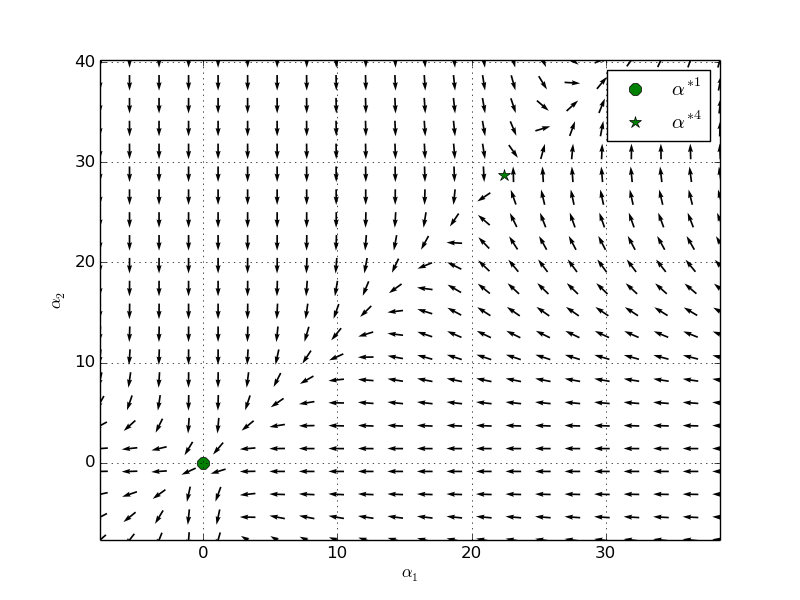
\includegraphics[scale = 0.7]{Python/plots/RG_flow/RG_flow3_2_6_0_2_0_1_0.png}
 \caption{Das Flussdiagramm für eine Lösung vom Typ \ref{Fall1b}. Der Fixpunkt 
  $\alpha^{*}_\text{vw}$ liegt im nicht-perturbativen Bereich. Die Parameter sind 
 $(\Nc,\Nd,\nfc,\nsc,\nfd,\nsd,\nfj,\nsj)=(3,2,6,0,2,0,1,0)$.}
 \label{fig:beta_QCDxdQCD:Sattelpunkt1}
\end{figure}


      An den Koeffizienten \eqref{eq:beta_QCDxdQCD:X1g} und 
      \eqref{eq:beta_QCDxdQCD:Y1g} sieht man, dass Skalare qualitativ den 
      gleichen Einfluss auf die $\beta$-Funktion wie Fermionen haben, 
      jedoch um einen Faktor $3$-$4$ kleiner, es ist also zu erwarten, dass 
      die Grenzen für die Anzahl der joint-Skalare um einen 
      entsprechenden Faktor höher liegen. Mögliche, Standardmodell nahe 
      Teilchenzahlen sind in Tabelle 
      \ref{tab:QCDxdQCD:Sattelpunkt_mit_Skalaren} zu sehen. 
      In Abbildung \ref{fig:beta_QCDxdQCD:Fix4_mit_Skalaren} ist außerdem 
      die Lage von $\alpha^{*}_\text{vw}$ für $0\leq \nsd \leq 3$ und $3\leq\nsj\leq 8$ 
      dargestellt. Hier ist zu erkennen, dass $\alpha^{*}_\text{vw}$ betragsmäßtig 
      kleiner wird, je mehr joint-Skalare eingeführt werden.

      \begin{table}
\centering

 \begin{tabular}{ccc|ccc}
 \toprule \midrule
$\Nd$ & $\nsd$ & $\nsj$ &	 $\Nd$ & $\nsd$ & $\nsj$	\\
\midrule
\multirow{5}{*}{2}& $0,1$& $3$-$9$    & \multirow{5}{*}{3} &$0$&$3$\\
 &  $2,3$& $3$-$8$ &  &$1$-$4$&$3,4$\\
 &  $4,5$&$3$-$7$  &  &$5-8$&$2,3,4$\\
 &  $6,7$&$3$-$6$ \\
 &  $8$&$3,4,5$\\    

  \midrule \bottomrule
 \end{tabular}
\caption{Mögliche Anzahlen von Skalaren für $\Nc=3$, $\nfc=6$, $\nfd=0$ .}
\label{tab:QCDxdQCD:Sattelpunkt_mit_Skalaren}
\end{table}

      \begin{figure}[h]
 \centering

 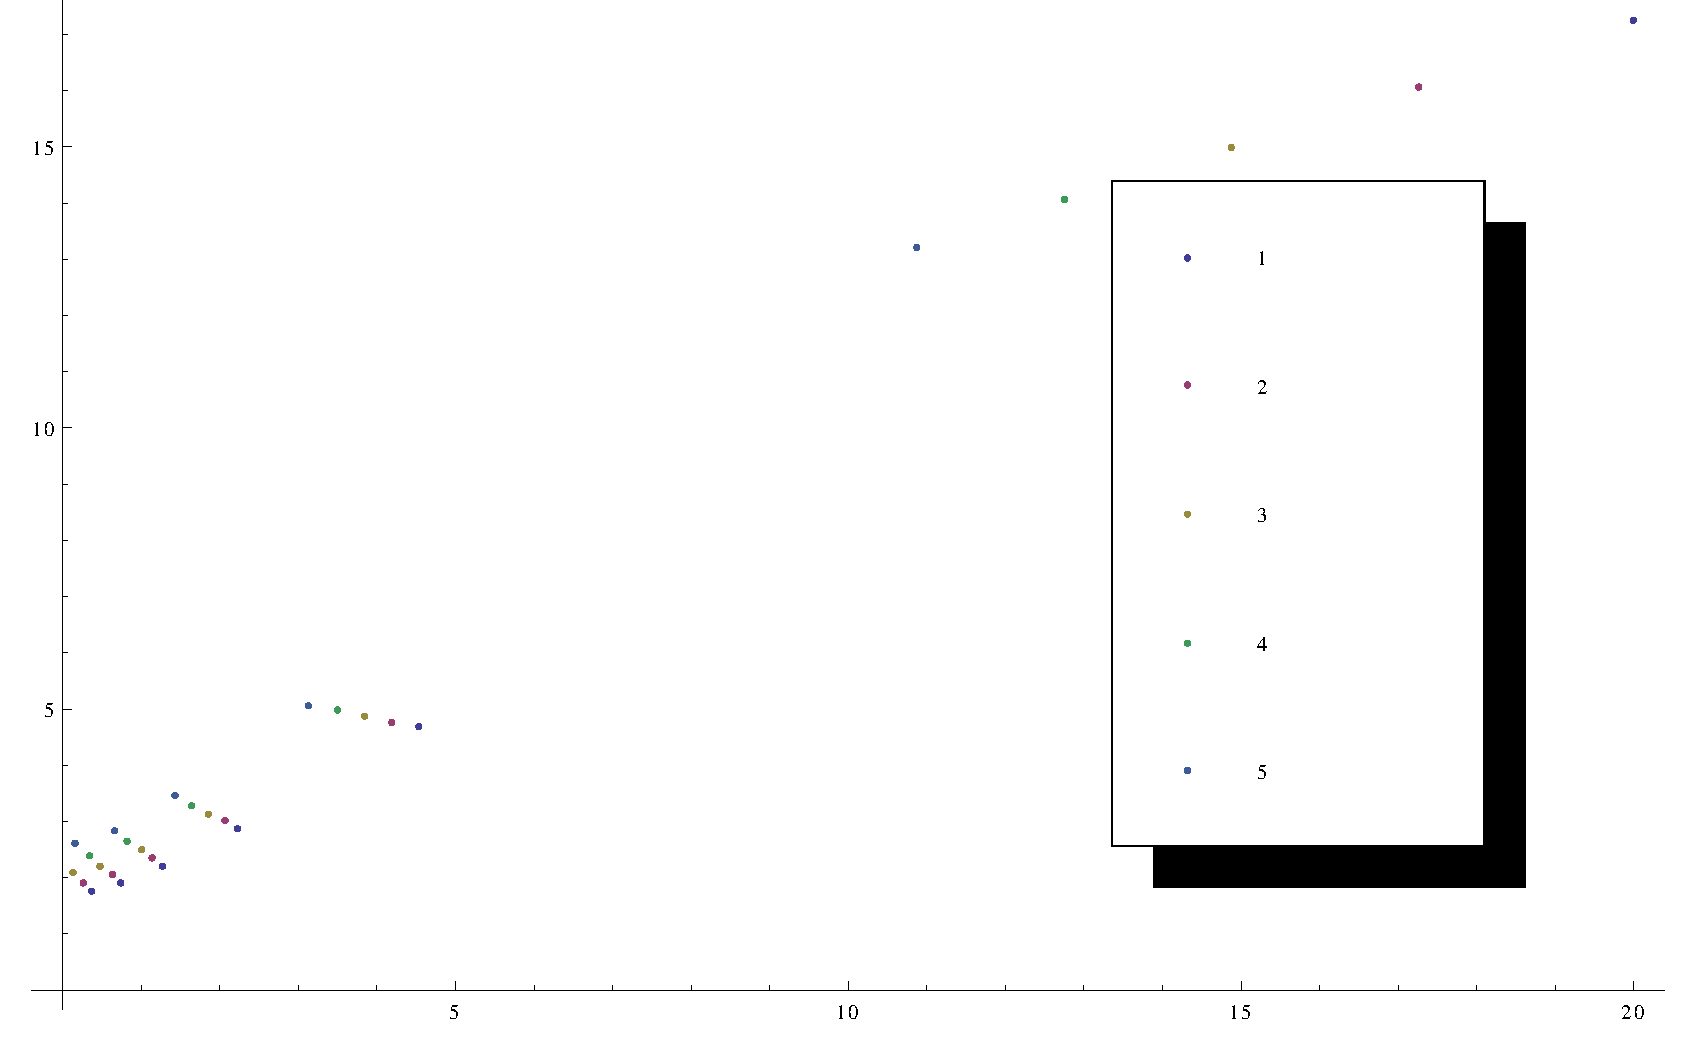
\includegraphics[scale = 0.5]{abschnitte/beta_QCDxdQCD/fig/Fix4_mit_Skalaren.pdf}

 \caption{Lage von $\alpha^{*4}$ in Abhängigkeit von $\nsd$ und $\nsj$.}
 
 \label{fig:beta_QCDxdQCD:Fix4_mit_Skalaren}

 \end{figure}

      
      Um einen vollständig wechselwirkenden UV-Fixpunkt zu erhalten, der mit 
      Methoden der Störungstheorie behandelt werden kann, ist es demnach 
      nötig, skalare Teilchen im joint-Sektor einzuführen. Die Teilchen des 
      dQCD-Sektors haben dagegen, wie in Abbildung 
      \ref{fig:beta_QCDxdQCD:Fix4_mit_Skalaren} zu sehen ist, nur geringe 
      Auswirkungen auf die Lage des Fixpunktes, ob hier Fermionen, Skalare oder 
      beide Teilchensorten eingeführt werden ist qualitativ nicht entscheidend.
      
      Wie in der Abbildung \ref{fig:beta_QCDxdQCD:Sattelpunkt1} zu sehen, 
      ist der Sattelpunkt $\alpha^{*}_\text{vw}$ in Richtung des Gaußschen Fixpunktes 
      $\alpha_\text{Gauß}^*$ UV-repulsiv. Bond und Litim haben gezeigt, dass dieses 
      Verhalten bei reinen Eichtheorien immer auftritt und schließen daraus, 
      dass es keine UV-Fixpunkte in reinen 
      Eichtheorien geben kann \cite{Bond_Litim}.
      In der Abbildung erkennt man, dass die zwei Trajektorien mit 
      $\alpha(t\to\infty)=\alpha^{*}_\text{vw}$ für 
      kleine Energien gegen 
      $\alpha^{*}_\text{tw2}$ bzw. $\alpha^{*}_\text{tw1}$, falls diese existieren, oder in 
      den nicht-perturbativen Bereich laufen. Hinsichtlich einer Erweiterung der 
      QCD, die im niederenergetischen Bereich durch das QCD-confinement 
      charakterisiert wird, können solche Trajektorien jedoch 
      physikalisch sinnvoll interpretiert werden. Um das genaue 
      Niederenergieverhalten zu erhalten müssten jedoch die Einflüsse der 
      Teilchenmassen berücksichtigt werden, in dieser Arbeit soll das aber nicht 
      geschehen.
      
  \subsection{UV-Verhalten bei $\alpha^{*}_\text{tw1}$}\label{beta_QCDxdQCD:UV_bei_Fix3}
    Da der Fixpunkt ein teilweise 
    wechselwirkender Fixpunkt ist, 
    muss hier das in \ref{beta_im_R2:nicht-hyperbolischer_Fixpunkt} 
    beschriebene Stabilitätskriterium angewendet werden. Zunächst kann aber 
    einfach gezeigt werden, dass dieser Fixpunkt nicht in jede Richtung 
    UV-attraktiv sein kann.
    
    Damit $\alpha^{*}_\s =-X_\s /Y_\s > 0$, muss $X_\s <0$ und $Y_\s >0$. Es wurde 
    in \ref{beta_QCDxdQCD:fix4:UV} gezeigt, das die umgekehrte Vorzeichenwahl 
    physikalisch nicht sinnvoll ist. Gleichung 
    \eqref{eq:beta_im_R2:stab_matrix_0} zeigt nun 
    $\lambda_1 =(\alpha^*_\s )^2 Y_\s > 0$ zu $e_1=(1,0)^\text{T}$, folglich muss 
    die $\alpha_\s$-Achse UV-repulsiv bezüglich $\alpha^{*}$ sein. 
    
    Am Fixpunkt ergibt sich aus \eqref{eq:beta_im_R2:lambda} und 
    \eqref{eq:beta_im_R2:stab_matrix_0} 
    \begin{equation}
     \lambda_2=0 \quad , \quad  e_2=\begin{pmatrix}
                            -Z_\s  /Y_\s \\ 1
                           \end{pmatrix}
                           \quad \text{und} \quad
    \quad \frac{\partial \lambda_2}{\partial \alpha_\d} = 2 X_\d
    -2\frac{X_\s}{Y_\s} Z_\d  \quad .
    \end{equation}
    Die Bedingung dafür, dass $\alpha^{*}$ ein Sattelpunkt ist, ist somit 
    \begin{equation}
     X_\s <0 \quad \land \quad Y_\s >0 \quad \land \quad X_\d Y_\s < Z_\d X_\s
     \quad . \label{eq:beta_QCDxdQCD:Bedingung3}
    \end{equation}
    Da die Vorzeichen $X_\s <0$, $Y_\s >0$ und $X_\d <0$ festgelegt sind, 
    kann bereits ohne Fallunterscheidung eine Grenze gefunden werden.
    Aus $X_\s <0 \land X_\d <0$ folgt allgemein (vgl. \eqref{Fall1b})
	\begin{equation}
	  \left(\nfj+\frac{1}{4} \nsj \right)^2 + \left( \nfj+\frac{1}{4}\nsj 
	  \right) \left( \nfd +\frac14 \nsd \right)\frac1\Nc 
	  + \frac{11}{2} \left(\nfc+\frac14 \nsc \right)\frac1\Nc < 
	  \left( \frac{11}{2} \right)^2 \quad \land \quad \text{c}
	  \leftrightarrow
	  \text{d} \quad. \label{eq:beta_QCDxdQCD:Fix3_ohne_Skalare}
	\end{equation}
   
    Zunächst werden wieder nur Fermionen betrachtet. Da sie außreichen, um 
    perturbative Fixpunkte zu modellieren, wird es nicht nötig sein, Skalare 
    einzuführen.
    Aus 
    \eqref{eq:beta_QCDxdQCD:Fix3_ohne_Skalare} und $X_\s <0$ folgen allgemeine 
    Grenzen für $\nfj$, $\Nd$ und $\nfd$
    \begin{equation}
    \begin{aligned}
     &\nfj < \sqrt{\left(\frac{11}{2}\right)^2-\frac{11}{2} \frac{\nfc}{\Nc}}
     =4.39
     \quad , \quad
     \nfd < \left(\left(\frac{11}{2}\right)^2 -1\right) \Nc -\frac{11}{2}
     \nfc = 54.75  \quad ,
     \\
     & \Nd<\frac{11}{2} \Nc -\nfc = 10.5      
    \end{aligned}
    \end{equation}
    für $\Nc=3$ und $\nfc=6$. 
    \begin{table}[h]
\centering
 \begin{tabular}{ccc|c||ccc|c}
 \toprule \midrule
 $\Nd$ 	& $\nfj$ 	& $\nfd$ 	& $\alpha^{*3}_1$ & $\Nd$ 	& $\nfj$ 	& $\nfd$ 	& $\alpha^{*3}_1$		 \\
 \midrule 
 $2$	& $2$		& $0$			& $2.21$  & $6$		& $1$	& $0$-$29$	& $0.75$	\\
 $3$	& $1$		& $0$-$8$		& $5.24$  & $7$		& $1$	& $0$-$35$	& $0.47$	\\
 $3$	& $2$		& $0$-$9$		& $0.85$  & $8$		& $1$	& $0$-$40$	& $0.28$	\\
 $3$	& $3$		& $0$-$7$		& $0.14$  & $9$		& $1$	& $0$-$46$	& $0.14$	\\
 $4$	& $1$		& $0$-$16$		& $2.21$  & $10$	& $1$	& $0$-$51$	& $0.04$	\\
 $4$	& $2$		& $0$-$15$		& $0.28$   		\\
 $5$	& $1$		& $0$-$23$		& $1.23$   		\\
 $5$	& $2$		& $0$-$21$		& $0.04$  		\\
 \midrule \bottomrule
 \end{tabular}
\caption{Mögliche Teilchenzahlen für einen Sattelpunkt bei $\alpha^{*3}$, mit $\Nc=3$, $\nfc=6$ und ohne Skalare.}
\label{tab:beta_QCDxdQCD:Fix3_ohne_Skalare}
\end{table}

    Tabelle \ref{tab:beta_QCDxdQCD:Fix3_ohne_Skalare} zeigt die möglichen 
    Teilchenanzahlen und die Komponente $\alpha^{*}_\s$. Im Gegensatz zum 
    vollständig wechselwirkenden Fixpunkt $\alpha^{*}_\text{vw}$ ist $\alpha^{*}_\text{tw1}$ 
    auch für eine Theorie ohne Skalare in einem perturbativ sinnvollen 
    Bereich, demnach können hier zwar wieder Skalare eingeführt werden, 
    ein neues Verhalten oder neue Wertebereiche für den Fixpunkt treten aber 
    nicht auf.
    

  \subsection{UV-Verhalten bei $\alpha^{*2}$}
    \begin{table}[h]
\centering
 \begin{tabular}{ccc||ccc}
 \toprule \midrule
 $\Nd$ 	& $\nfj$ 	& $\nfd$ 	 & $\Nd$ 	& $\nfj$ 	& $\nfd$ 			 \\
 \midrule 
 $2$	& $1$		& $3$-$7$		& $5$		& $1$	& $13$-$24$	\\
 $2$	& $2$		& $1$-$4$		& $5$		& $2$	& $19$-$21$	\\
 $2$	& $3$		& $0$-$1$		& $6$		& $1$	& $17$-$29$	\\
 $3$	& $1$		& $6$-$13$		& $7$		& $1$	& $22$-$35$	\\
 $3$	& $2$		& $4$-$10$		& $8$		& $1$	& $28$-$40$	\\
 $3$	& $3$		& $4$-$7$		& $9$		& $1$	& $36$-$46$	\\
 $4$	& $1$		& $9$-$18$		& $10$		& $1$	& $47$-$51$	\\
 $4$	& $2$		& $10$-$15$		\\
 \midrule \bottomrule
 \end{tabular}
\caption{Mögliche Teilchenzahlen für einen Sattelpunkt bei $\alpha^{*}_\text{tw2}$, mit $\Nc=3$, $\nfc=6$ und ohne Skalare.}
\label{tab:beta_QCDxdQCD:Fix2_ohne_Skalare}
\end{table}

    Aufgrund der Symmetrie der $\beta$-Funktion in den Indizes $\text{c}$ und 
    $\text{d}$ bzw. $1$ und $2$ ist das allgemeine Vorgehen wie bei $\alpha^{*}_\text{tw1}$. Der Fixpunkt 
    ist in $\alpha_\d$-Richtung repulsiv und das Kriterium für einen Sattelpunkt 
    analog zu \eqref{eq:beta_QCDxdQCD:Bedingung3} 
    \begin{equation}
     X_\d <0 \quad \land \quad Y_\d >0 \quad \land \quad X_\s Y_\d < Z_\s X_\d
     \quad .
    \end{equation}
    Ähnlich wie bei Fixpunkt $\alpha^{*}_\text{tw1}$ ist es auch bei $\alpha^{*}_\text{tw2}$ nicht 
    nötig Skalare einzuführen, da sie zu keinem qualitativ neuen Verhalten 
    führen. Wieder gibt es Ober- und Untergrenzen für $\Nd$, $\nfj$ und 
    $\nfd$ um eine UV-attraktive Richtung zu erhalten. Die 
    möglichen Werte sind in Tabelle \ref{tab:beta_QCDxdQCD:Fix2_ohne_Skalare} 
    zu sehen.
    
    
  \subsection{Qualitative Änderungen durch Yukawa-Terme}
    \begin{figure}[h]
%\centering
\begin{minipage}[t]{0.5 \textwidth}
 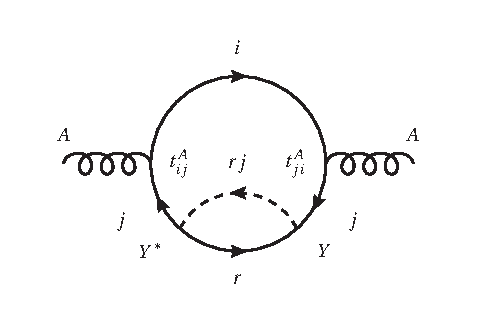
\includegraphics{abschnitte/beta_QCDxdQCD/fig/Yukawa1.eps}
 \caption*{(a)}
\end{minipage}
\begin{minipage}[t]{0.5\textwidth}
 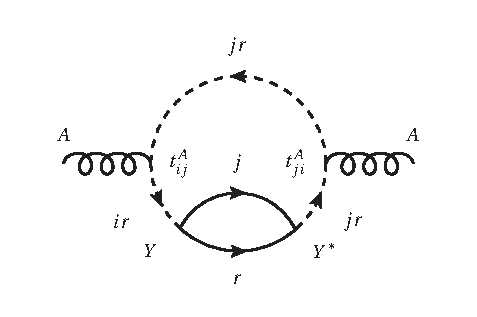
\includegraphics{abschnitte/beta_QCDxdQCD/fig/Yukawa2.eps}
 \caption*{(b)}
 \end{minipage}
 \begin{minipage}[t]{0.5\textwidth}
 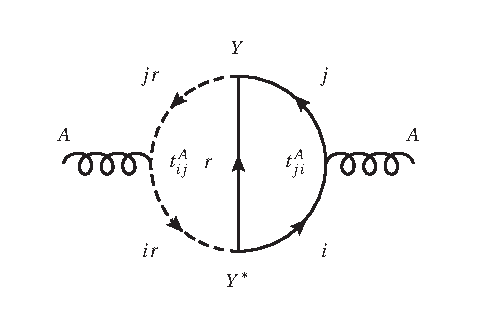
\includegraphics{abschnitte/beta_QCDxdQCD/fig/Yukawa3.eps}
 \caption*{(c)}
 \end{minipage}
\caption{Yukawa-Beiträge zum Gluonpropagator.}\label{fig:beta_QCDxdQCD:Yukawa}
 \end{figure}
    In \cite{Asymptotic_safety_guaranteed} schließen Litim und Sannino, dass 
    Yukawa-Kopplungen nötig sind, um in einer (einfachen) Eich-Yukawa-Theorie 
    nicht-triviale UV-Fixpunkte zu erzeugen. Bond und Litim haben 
    dies auch für allgemeine Eich-Yukawa-Theorien mit 
    ungeladenen Skalaren gezeigt \cite{Bond_Litim}. Damit haben sie 
    insbesondere gezeigt, dass ein UV-repulsiver Gaußscher Fixpunkt mit 
    einer Trajektorie zum wechselwirkenden Sattelpunkt $\alpha^{*}_\text{vw}$ nur durch 
    Hinzunahme von Yukawa-Kopplungen möglich ist. Wie bisher gezeigt, können 
    UV-attraktive Richtungen für wechselwirkende Fixpunkte auch in 
    reinen Eichtheorien enstehen. Es soll nun eine qualitative Abschätzung 
    gegeben werden, auf welche Weise mögliche Yukawa-Wechselwirkungen die 
    Eigenschaften der bisher gefundenen Fixpunkte verändern.
    
    Wie in Abschnitt \ref{QCDxdQCD} beschrieben gibt es nur eine eine Art der 
    Yukawa-Kopplung, Gleichung \eqref{eq:QCDxdQCD:Yukawa_misch}, die mit nur 
    einer Kopplungskontstanten auskommt, und deshalb für veränderliche 
    Flavour-Zahlen einfach untersucht werden kann. Der Beitrag zur 
    $\beta$-Funktion der Eichkopplungen wurde von Machacek und Vaughn 
    als
    \begin{equation}
     \beta^\text{Yukawa}_\s(g) = -g_\s^3(16 \uppi^2)^{-2} \frac{2}{d(G)} 
     \left[ C_2(R_\s) \delta^{il} Y^{l,r,js}(Y^{i,r,js})^*\right]
     \label{eq:beta_QCDxdQCD:beta_g_Yukawa}
    \end{equation}
    berechnet \cite{MACHACEK198383}. Sie haben außerdem festgestellt, dass nur 
    das Diagramm \ref{fig:beta_QCDxdQCD:Yukawa}(a) zur $\beta$-Funktion 
    beiträgt. Mit \eqref{eq:QCDxdQCD:Yukawa_Struktur} lässt sich 
    \eqref{eq:beta_QCDxdQCD:beta_g_Yukawa} zu
    \begin{align}
     \beta^\text{Yukawa}_\s(g) &=
     -g_\s^3|Y|^2 (16 \uppi^2)^{-2}\frac{2 C_2(R_\s) d(R_\s) d(R_\d)}{d(SU(\Nc))} 
     \nsj\\
     &= -g_\s^3|Y|^2(16 \uppi^2)^{-2} \nfc\nfd\nsj \Nd
    \end{align}
    zusammenfassen. Bemerkenswert ist hierbei, dass wegen 
    \begin{equation}
     C_2(R) d(R) = T(R)d(G) \quad , \quad T(R)=\nicefrac{1}{2}\,\,\,\text{
     für $SU(N)$}
    \end{equation}
    der Yukawa-Term in $\beta_\s$ unabhängig von $\Nc$ ist. Dies ist darauf 
    zurückzuführen, dass QCD- und joint-Teilchen gleich unter der $SU(\Nc)$ 
    transformieren. Mit $\alpha_Y:=\nicefrac{|Y|^2}{4\uppi}$ und 
    \begin{equation}
     A_\s :=\frac{2}{16\uppi^2} \nfc\nfd\nsj \Nd \quad \text{sowie} \quad
     A_\d :=\frac{2}{16\uppi^2} \nfc\nfd\nsj \Nc \quad 
    \end{equation}
    wird \eqref{eq:beta_QCDxdQCD:beta_alpha} zu 
    \begin{equation}
   \begin{pmatrix}
    \beta_\s(\alpha) \\ \beta_\d(\alpha)
   \end{pmatrix}
    = 
    \begin{pmatrix}
       X_\s \alpha_\s^2 + Y_\s \alpha_\s^3 + Z_\s \alpha_\s^2 \alpha_\d -
       A_\s\alpha_\s^2\alpha_Y\\ 
       X_\d \alpha_\d^2 + Y_\d \alpha_\d^3 + Z_\d \alpha_\s \alpha_\d^2-
       A_\d \alpha_\d^2 \alpha_Y
                    \end{pmatrix}
     \label{eq:beta_QCDxdQCD:beta_alpha_Yukawa} \quad .
  \end{equation}
  Auch ohne die explizite $\beta$-Funktion für die Yukawa-Kopplung lassen sich 
  bereits qualitative Einflüsse auf die Lage der Fixpunkte ableiten.
  Als Erweiterung zu $\alpha^{*}_\text{tw1}$ (vgl. \eqref{eq:beta_QCDxdQCD:Fixpunkte}) 
  können die Fixpunkte
  \begin{equation}
   \widehat{\alpha}^*=\left(-\frac{X_\s}{Y_\s},0,0\right) 
   \quad \text{und} \quad 
   {\alpha}^*=\left(\alpha_\s^*,0, \alpha_Y^*\right)
  \end{equation}
  gefunden werden.
%   Dabei stellt $\widehat{\alpha}^*$ die triviale Erweiterung des 
%   Yukawa-freien Falls dar. 
  Aus 
  \eqref{eq:beta_QCDxdQCD:beta_alpha_Yukawa} folgt 
  \begin{equation}
   X_\s + Y_\s \alpha_\s^* -A_\s \alpha_Y^*=0  \label{eq:beta_QCDxdQCD:Yukawa_a2}
   \quad\Rightarrow\quad
   \alpha_\s^*> - \frac{X_\s}{Y_\s} = \widehat{\alpha}_\s^* \quad ,
  \end{equation}
  wobei $A_\s>0$ und $\alpha_Y^*>0$ ausgenutzt wurde. Auf ähnliche Weise kann 
  für den vollständig wechselwirkenden Fixpunkt $\alpha^{*}_\text{vw}$ verfahren 
  werden. Für die Fixpunkte
  \begin{equation}
   \widehat{\alpha}^*=\left( \frac{Z_\s X_\d -X_\s Y_\d}{Y_\s Y_\d -Z_\s Z_\d},
   \frac{Z_\d X_\s -X_\d Y_\s}{Y_\s Y_\d-Z_\s Z_\d},0\right) 
   \quad \text{und} \quad 
   {\alpha}^*=\left(\alpha_\s^*,\alpha_\d^*, \alpha_Y^*\right) 
   \label{eq:beta_QCDxdQCD:Yukawa_a4}
  \end{equation}
  folgt 
  \begin{equation}
   \alpha_\s^*>\widehat{\alpha}_\s^* \quad \text{und} \quad 
   \alpha_\d^*>\widehat{\alpha}_\d^* \quad .
  \end{equation}
  Man erkennt, dass eine Yukawa-Kopplung mit $\alpha_Y(t\to\infty)\neq 0$ die 
  Kopplungskonstanten $\alpha_\s^*$ und $\alpha_\d^*$ stets vergrößert. Hier 
  ist eine genaue Berechnung von $\beta_Y$ nötig, um zu überprüfen ob  
  $\alpha_\s^*$ und $\alpha_\d^*$ weiterhin im perturbativen Bereich liegen 
  können. Hinsichtlich Abbildung \ref{fig:beta_QCDxdQCD:Fix4_mit_Skalaren} 
  ist zu erwarten, dass die Untergrenze für $\nsj$ um physikalische und 
  perturbative Fixpunkte zu erhalten durch die nicht verschwindende 
  Yukawa-Kopplung erhöht wird. An \eqref{eq:beta_QCDxdQCD:Yukawa_a2} bzw. 
  \eqref{eq:beta_QCDxdQCD:Yukawa_a4} erkennt man außerdem
  \begin{equation}
   \alpha_Y^*=\frac{X_\s +Y_\s \alpha_\s^*+Z_\s \alpha_\d^*}{A_\s} 
   \left( = \frac{X_\d+Y_\d\alpha_\d^*+Z_\d \alpha_\s^*}{A_\d} \right) \quad .
  \end{equation}
  Da $X_\s$, $Y_\s$ und $Z_\s$ unabhängig von $\nfd$ sind währen $A_\s \propto \nfd$, 
  lässt sich vermuten, dass eine hohe Anzahl von dQCD-Fermionen die 
  Perturbativität von $\alpha_Y$ begünstigt, unter der Annahme, dass sich 
  $\alpha_\s^*$ und $\alpha_\d^*$ ähnlich verhalten wie im Yukawa-freien Fall.
  
 


  
